\chapter{Windows 11 修整指南}
\label{windows-11-optimization}

\begin{intro}
  2021 年 10 月 5 日,微软发布了\CJKsout*{又新又好}的 Windows 11。在那之后,许多品牌的笔记本电脑和台式机开始出厂即预装这款新系统,一些原本使用 Windows 10 的同学也在微软的蛊惑之下升级到了 Windows 11。

  一方面,Windows 11 在外观和部分使用体验上有着不小进步;但另一方面,Windows 11 在很多地方都让人「火大」——性能损失、花式 bug、部分操作反人类……为了让现阶段的 Windows 11 变得更好用一些,我们总结了一些对 Windows 11 系统进行「修整」的方法和技巧,以供大家参考使用。
\end{intro}

\begin{note}
  本章会持续更新,其中的内容会随着时间推移而有所增删。
\end{note}

\begin{warning}
  由于 Windows 更新频繁,这部分介绍的各种技巧都可能随时失效。

  此外,这部分介绍的技巧中,有不少都需要更改系统底层的一些选项,若操作不当可能造成意料之外的后果,因而操作前请三思。
\end{warning}

\section{使用旧版右键菜单}

Windows 11 在「文件资源管理器」(包括桌面)中引入了一套新的右键菜单,如图 \ref{New_menu} 所示。

\begin{figure}[htb!]
  \centering
  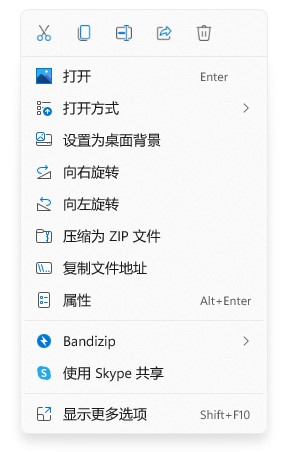
\includegraphics[width=6cm]{assets/New_menu.jpg}
  \caption{Windows 11 的新式右键菜单}
  \label{New_menu}
\end{figure}

这套新的右键菜单虽然相比旧式菜单略显美观,但在很多时候并不实用:先不说这个新式菜单 bug 超级多,由于今天的大多数应用仍然没有接入这套新的菜单系统,很多时候我们不得不在右键后点选【显示更多选项】这一项来打开旧式菜单以找到我们需要的功能。因此,在新式菜单成熟之前,我们可以通过下面的方法来始终使用旧式菜单。

设置的方法如下:

\begin{itemize}
  \item 按 \keys{ + X},选择【Windows 终端(管理员)】,然后选择【是】。(部分机器上称「Windows Powershell(管理员)」)
  \item 输入这行命令,然后按一次回车。重启后即见效果:
  \begin{lstlisting}
    reg add "HKCU\Software\Classes\CLSID\{86ca1aa0-34aa-4e8b-a509-50c905bae2a2}\InprocServer32" /f /ve
  \end{lstlisting}
\end{itemize}

这样设置之后,在文件资源管理器(包括桌面)中右键,都将继续使用旧式菜单,如图 \ref{Old_menu} 所示。

\begin{figure}[htb!]
  \centering
  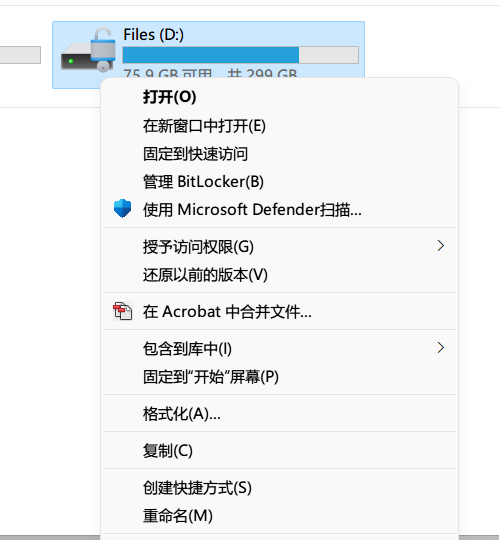
\includegraphics[width=7cm]{assets/Old_menu.png}
  \caption{操作之后,将换回原来的旧式右键菜单}
  \label{Old_menu}
\end{figure}

如果需要返回新版菜单,使用下面这行命令:

\begin{lstlisting}
  reg delete "HKCU\Software\Classes\CLSID\{86ca1aa0-34aa-4e8b-a509-50c905bae2a2}" /f
\end{lstlisting}
